En la Figura~\ref{fig:model_loss} se muestra la el valor de la p\'erdida MSE en funci\'on de la \'epoca de entrenamiento. \\

El mejor modelo de obtiene despu\'es de 184 \'epocas, con un valor de p\'erdida para el conjunto de datos de entrenamiento de 49605.3, para el conjunto de datos de validaci\'on de 50399.8, y para el conjunto de datos de testeo de 53731.6.  \\

\begin{figure}[h]
\centering
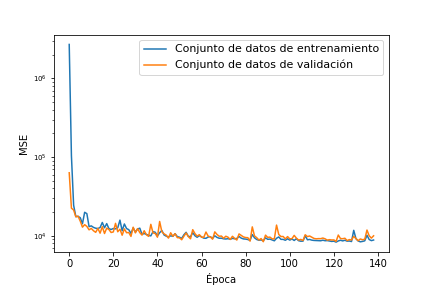
\includegraphics[width=0.8\textwidth]{figures/model_loss.png}
\caption{Valor del MSE en funci\'on de la \'epoca de entrenamiento para el conjunto de datos de entrenamiento (en azul) y para el conjunto de datos de validaci\'on (en naranja).}
\label{fig:model_loss}        
\end{figure}


En la Figura~\ref{fig:R_predicted} se comparan la distribuciones de la resoluci\'on R, definida en \eqref{eq:R}, calculadas sobre el conjunto de datos de testeo a partir del $p_{T}$ que da el algoritmo TuneP y a partir del $p_{T}$ que predice la red neuronal respectivamente. \\

\begin{figure}[h]
\centering
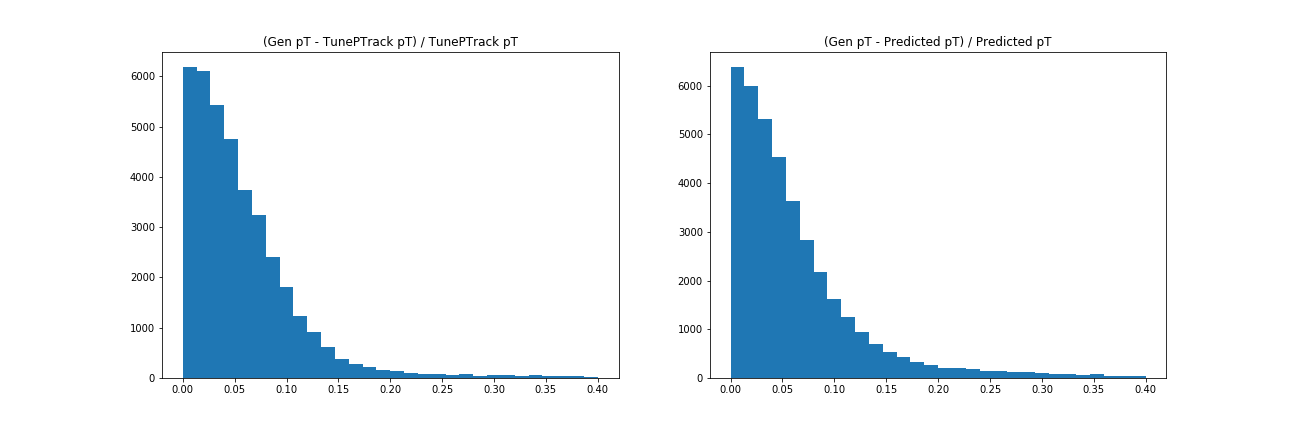
\includegraphics[width=1.1\textwidth]{figures/R_predicted.png}
\caption{Distribuci\'on de la resoluci\'on R dada por \eqref{eq:R} sobre el conjunto de datos de testeo. Izquierda: tomando el $p_{T}$ que da el algoritmo TuneP. Derecha: tomando el $p_{T}$ predicho por el modelo de regresi\'on al $p_{T}$.}
\label{fig:R_predicted}        
\end{figure}

Por \'ultimo, en la Figura~\ref{fig:ptpred_tuneppt} se muestra la distribuci\'on bidimensional del momento transverso de predicho por la red en funci\'on del momento transverso de generaci\'on para los muones del conjunto de datos de testeo. \\

\begin{figure}[h]
\centering
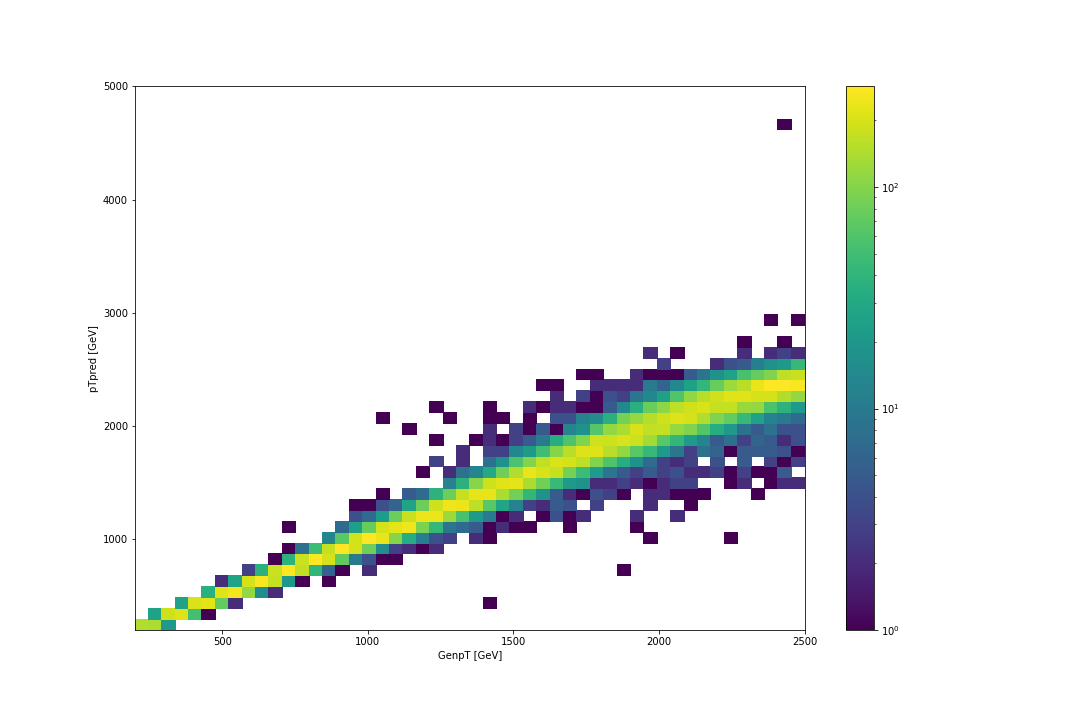
\includegraphics[width=1.0\textwidth]{figures/data_test_ptpred_genpt.png}
\caption{Distribuci\'on bidimensional del $p_{T}$ predicho por la red neuronal en funci\'on del $p_{T}$ de generaci\'on para los muones del conjunto de datos de testeo.}
\label{fig:ptpred_tuneppt}  
\end{figure}



\clearpage
